\documentclass{beamer}

\mode<presentation> {

\usetheme{Berkeley}
\usecolortheme{lily}


}
\usepackage{amsmath,amsfonts,amssymb}
\usepackage{gensymb}
\usepackage{graphicx} % Allows including images
\usepackage{booktabs} % Allows the use of \toprule, \midrule and \bottomrule in tables

%----------------------------------------------------------------------------------------
%	TITLE PAGE
%----------------------------------------------------------------------------------------

\title[Matrix Project]{EE1390 - Intro to AI and ML}

\author{Yogesh Swami\inst{1} \and Sahir Bansal\inst{2}} % Your name
\institute[IIT Hyderabad]
{
  \inst{1}%
  EP17BTECH11019
  \and
  \inst{2}%
  EE17BTECH11035
}
\date{\today} % Date, can be changed to a custom date

\subject{Analysis}
\AtBeginSubsection[]
{
  \begin{frame}<beamer>{Analysis}
    \tableofcontents[currentsection,currentsubsection]
  \end{frame}
}

\begin{document}

\begin{frame}
\titlepage % Print the title page as the first slide
\end{frame}


\begin{frame}{Matrix problem in coordinate geometry}{From 2011 JEE(Advanced)[Paper 1 - Q53]}
  \begin{itemize}
\item A straight line L through the point (3,-2) is inclined at an angle $60\degree$ to the line $\sqrt{3}x +y = 1$ . If L also intersects x-axis, then find the equation of L.
\\
  .
  \end{itemize}
\end{frame}


\begin{frame}
\frametitle{Problem Solving Strategy} % Table of contents slide, comment this block out to remove it
\tableofcontents % Throughout your presentation, if you choose to use \section{} and \subsection{} commands, these will automatically be printed on this slide as an overview of your presentation
\end{frame}

%----------------------------------------------------------------------------------------
%	PRESENTATION SLIDES
%----------------------------------------------------------------------------------------



%------------------------------------------------
\section{Theoretical Computation} % Sections can be created in order to organize your presentation into discrete blocks, all sections and subsections are automatically printed in the table of contents as an overview of the talk
%------------------------------------------------


\subsection{Using Matrix} % A subsection can be created just before a set of slides with a common theme to further break down your presentation into chunks

\begin{frame}
\frametitle{Solution in matrix form}
\begin{itemize}
\item Given $L\textsubscript{1}$ : $\sqrt{3}x +y = 1$
\item Given point \textbf{C} &= \begin{bmatrix}
           3 \\
           -2 \\
  \end{bmatrix}
\end{itemize}
\end{frame}

%------------------------------------------------

\begin{frame}
\frametitle{Solution in matrix form:(contd)}
\begin{itemize}
\item For the given line $L\textsubscript{1}$
\item x-intercept = {\dfrac{1}{\sqrt{3}}}
\\ \item y-intercept = 1
\\ \item So, this line passes through points $\textbf{P}$ and $\textbf{Q}$
\\where \textbf{P} &= \begin{bmatrix}
           0 \\
           1 \\
  \end{bmatrix}
  and
  \textbf{Q} &= \begin{bmatrix}
           {\dfrac{1}{\sqrt{3}}} \\
           0 \\
  \end{bmatrix}
  
\\ \item Now, horizontally stacking $\textbf{P}$ and $\textbf{Q}$ , we get matrix $\textbf{A}$,
\\where \textbf{A} &= \begin{bmatrix}
           0 & {\dfrac{1}{\sqrt{3}}} \\
           1 & 0 \\
  \end{bmatrix}
\end{itemize}
\end{frame}

%------------------------------------------------

\begin{frame}
\frametitle{Solution in matrix form:(contd)}
\begin{itemize}
    \item Now the given line $L\textsubscript{1}$ is rotated by angle $60\degree$ such that it passes through $\textbf{C}$.
    \item Now, pre-multiplying $\textbf{A}$ with rotation matrix $\textbf{R}$,
\\where \textbf{R} &= \begin{bmatrix}
           cos\theta & sin\theta \\
           -sin\theta & cos\theta \\
  \end{bmatrix}
  \item Here, $\theta$ is rotation angle i.e. $60\degree$ .
  \item $\therefore$ \textbf{R} &= \begin{bmatrix}
           \dfrac{1}{2} & \dfrac{\sqrt{3}}{2} \\
           \dfrac{-\sqrt{3}}{2} & \dfrac{1}{2} \\
  \end{bmatrix}
\end{itemize}
\end{frame}

%------------------------------------------------

\begin{frame}
\frametitle{Solution in matrix form:(contd)}
\begin{itemize}
    \item So, $\textbf{A'}$ = $\textbf{R}$.$\textbf{A}$
    \item $\textbf{A'}$ = \begin{bmatrix}
           \dfrac{1}{2} & \dfrac{\sqrt{3}}{2} \\
           \dfrac{-\sqrt{3}}{2} & \dfrac{1}{2} \\
  \end{bmatrix}   \begin{bmatrix}
           0 & {\dfrac{1}{\sqrt{3}}} \\
           1 & 0 \\
  \end{bmatrix}
  \item $\therefore$ \textbf{A'} &= \begin{bmatrix}
           \dfrac{\sqrt{3}}{2} & \dfrac{1}{2\sqrt{3}} \\
           \dfrac{1}{2} & \dfrac{-1}{2} \\
  \end{bmatrix}
\end{itemize}
\end{frame}

%------------------------------------------------
%------------------------------------------------

\begin{frame}
\frametitle{Solution in matrix form:(contd)}
\begin{itemize}
    \item Now, splitting $\textbf{A'}$ into $\textbf{P'}$ and $\textbf{Q'}$
    \\where $\textbf{P'}$ and $\textbf{Q'}$ are rotated vectors of $\textbf{P}$ and $\textbf{Q}$
    \item $\therefore$ \textbf{P'} &= \begin{bmatrix}
           \dfrac{\sqrt{3}}{2} \\
           \dfrac{1}{2}  \\
  \end{bmatrix} and \textbf{Q'} &= \begin{bmatrix}
           \dfrac{1}{2\sqrt{3}} \\
           \dfrac{-1}{2} \\
  \end{bmatrix}
  \item Consider $\textbf{M}$ = $\textbf{P'}$ - $\textbf{Q'}$
  \\where $\textbf{M}$ is the direction vector of required line L .
  \item $\therefore$ \textbf{M} &= \begin{bmatrix}
           \dfrac{1}{\sqrt{3}} \\
           1  \\
  \end{bmatrix}
\end{itemize}
\end{frame}

%------------------------------------------------

%------------------------------------------------

\begin{frame}
\frametitle{Solution in matrix form:(contd)}
\begin{itemize}
    \item As we know the direction vector. Now, we can the find normal vector $\textbf{n}$ by equation : $\mathbf{n}^\intercal$$\textbf{M}$ = 0
    \item $\textbf{n}$ = \begin{bmatrix}
           0 & 1 \\
           -1 & 0 \\
  \end{bmatrix} $\textbf{M}$
    \item $\textbf{n}$ = \begin{bmatrix}
           0 & 1 \\
           -1 & 0 \\
  \end{bmatrix} \begin{bmatrix}
           \dfrac{1}{\sqrt{3}} \\
           1  \\
  \end{bmatrix}
  
    \item $\textbf{n}$ = \begin{bmatrix}
           1 \\
           \dfrac{-1}{\sqrt{3}} \\
  \end{bmatrix}
\end{itemize}
\end{frame}

%------------------------------------------------


%------------------------------------------------

\begin{frame}
\frametitle{Solution in matrix form:(contd)}
\begin{itemize}
    \item Now, we have Normal vector of required line as well as a point on the line.
    \item So, we can now write the equation of line L as :
    \\ $\mathbf{n}^\intercal$($\textbf{X}$ - $\textbf{C}$) = 0
    \item \begin{bmatrix}
           1 & \dfrac{-1}{\sqrt{3}}
  \end{bmatrix}\begin{bmatrix}
           x-3 \\
           y+2 \\
  \end{bmatrix} = 0
  \item On solving this , we get equation of required line:
  \\ y - $\sqrt{3}$x + 2 + 3$\sqrt{3}$ = 0 
\end{itemize}
\end{frame}


%------------------------------------------------
\section{Graphical Verification}
\subsection{Using Python}



%------------------------------------------------

\begin{frame}{Python code}
Python Code Used
 \centering
\includegraphics[scale=0.4]{code.png}

\end{frame}


\begin{frame}{Figure}
Figure generated by python code
 \centering
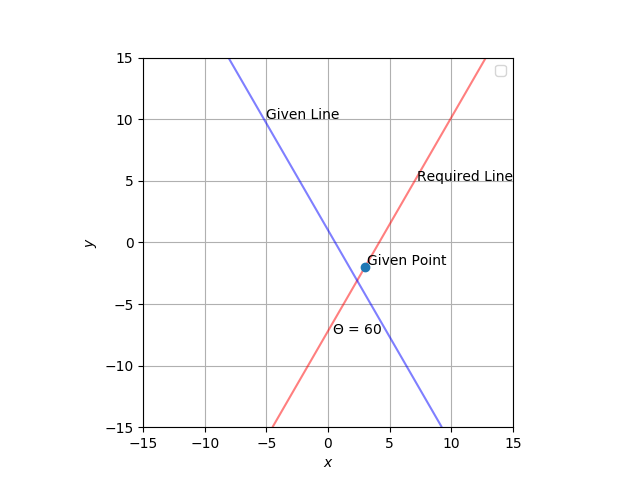
\includegraphics[scale=0.6]{Matrix.png}

\end{frame}


\begin{frame}
\Huge{\centerline{Thank you}}
\end{frame}


%----------------------------------------------------------------------------------------

\end{document}
